% infolim.tex

% why is there a limit?
\begin{frame}
    \frametitle{Information Theoretic Limits}

    
    \begin{multicols}{2}
        
        \begin{figure}
            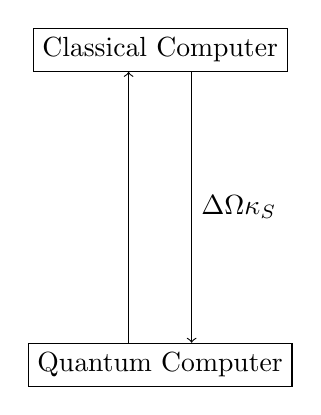
\begin{tikzpicture}[node distance = 4cm]
                \node[draw, rectangle] (C) {Classical Computer};
                \node[draw, rectangle, below of=C] (Q) {Quantum Computer};
	
                
                \begin{scope}[transform canvas={xshift=0.4cm}]
                \draw[->] (C) -- node[right, midway] {$\Delta\Omega \kappa_S$} (Q);
                \end{scope}
                
                \begin{scope}[transform canvas={xshift=-0.4cm}]
                    \draw[->] (Q) -- node[below, midway] {} (C);
                \end{scope}
            \end{tikzpicture}
        \end{figure}
        %
        The classical system transferring information about the parameters to
        the PQC has a limit on how much information it can transfer in a given
        time \(T\) given by
        \begin{gather*}
            b = T\Delta\Omega\kappa_s
        \end{gather*}
        where \(\Delta\Omega\) is the channel bandwidth and \(\kappa_s\) is the
        bit depth of the control signal (amount of information \emph{per}
        trasnfer).
    \end{multicols}

\end{frame}

% summary of bounds on qoc
\begin{frame}
    \frametitle{Example --- Bounds on Quantum Optimal Control}

    For the specific example of a control pulse for a quantum system
    \cite{lloyd2014information}

    \begin{gather*}
        \dot{\rho} = \mathcal{L}(\rho, \gamma(t))~,
    \end{gather*}

    where \(\rho\) is the state density matrix, \(\mathcal{L}\) is the
    Liouvillian operator, and \(\gamma(t)\) is the control pulse. We have the
    Hamiltonian

    \begin{gather*}
        \hamiltonian = \hamiltonian_D + \gamma(t)\cdot \hamiltonian_C~.
    \end{gather*}

\end{frame}

\begin{frame}
    \frametitle{Example --- Bounds on Quantum Optimal Control}
    
    We have

    \begin{gather*}
        \kappa_s = \log (1 + \frac{\Delta\gamma}{\delta\gamma})~,
    \end{gather*}

    where \(\Delta\gamma\) and \(\delta\gamma\) are the maximum and minimum
    variation in the control field.

    We have the error bound \footfullcite{lloyd2014information}
    \(\norm*{\rho-\rho_*} > \epsilon\), with

    \begin{gather*}
        \epsilon \geq 2^{-\frac{T\Delta\Omega\kappa_s}{\dimD_\polyreachable}}~,
    \end{gather*}

    where \(\dimD_\polyreachable\) is the dimension of the relevant
    (polynomially reachable) space of density matrices.

    \notes{We intend to employ a similar analysis to establish bounds on PQC errors.}

\end{frame}

\begin{frame}
    \frametitle{Parameter Space Dimension - Fisher Information}

    \begin{gather}
        \left[ F_\mu (\parameters)\right] = 
                4\text{Re}
                \left[
                    \braket{\partial_i \psi_\mu(\parameters)}{\partial_j \psi_\mu(\parameters)}
                % \qquad\qquad
                % \right.\nonumber\\
                % \left. \qquad\qquad
                    -
                    \braket{\partial_i \psi_\mu(\parameters)}{\psi_\mu(\parameters)}
                    \braket{\psi_\mu(\parameters)}{\partial_j \psi_\mu(\parameters)}
                \right]
    \end{gather}

    where \(\psi_\mu\) varies over the input state set.

    \(F_\mu\) is \(M\times M\) where \(M\) is the number of parameters in the
    control. \\

    \pause
    
    \begin{center}
        \emph{Increase M till rank plateaus.}
    \end{center}

    \notes{Question: What does this Mmax look like then?}

\end{frame}

\begin{frame}
    \frametitle{Parameter Scaling Bounds}

    \notes{Some suggestions have been made that polynomially growing parameter space
    anstazes can be used for VQAs. But the work is speculative and it remains to
    be seen whether any interesting problems fall within this class of 2-design
    solvability.}

    \begin{multicols}{2}
        
        \begin{center}
            \includegraphics<1>[width=0.5\textwidth]{figures/linear.pdf}
            \includegraphics<2>[width=0.5\textwidth]{figures/poly.pdf}
            \includegraphics<3>[width=0.5\textwidth]{figures/exp.pdf}
        \end{center}
        %
        \begin{itemize}
            \item<1-> Linear?
            \item<2-> Polynomial?
            \item<3-> Exponential, in general.
        \end{itemize}
    \end{multicols}

\end{frame}

\begin{frame}
    \frametitle{Trainability Tradeoff}

    What problems does this bring?
    \pause
    
    \begin{gather}
        \epsilon \geq e^{-\frac{T\Delta\Omega\kappa_S}{\dimD_{\polyreachable}}}~,\\
        T\Delta\Omega\kappa_S \geq \dimD_{\polyreachable}\ln(\frac{1}{\epsilon})~.
    \end{gather}

\end{frame}

\begin{frame}
    \frametitle{Consequences?}

    \begin{itemize}[<+->]
        \item Not a complexity bound! \footfullcite{bittel2021trainingvqa}
        \item Specification constraints!
    \end{itemize}

    \notes{While training of VQAs being NP-Hard has been discussed, quantum variational
    eigensolvers and approximate optimization algorithms have been understood to
    be heuristics, and it is generally fine if the worst case complexity is bad,
    as long as for most problems you have something nice.}

    \notes{However, this is a hardware constraint. To be able to ensure we explore the
    correct solution space, designers will have to provision higher bandwidth
    devices for all test cases, and as such we think this may have serious
    consequences for design and applicability of variational quantum algorithms. }

\end{frame}

% % bounds on qsvm
% \begin{frame}
%     \frametitle{Quantum SVM}

%     Given training data embedded as n-qubit quantum states \(\{\ket*{x_i}\}\) with
%     corresponding labels \({y_i = \pm 1}\), a QSVM implemented as a VQA attempts to learn a
%     unitary \(\pqc(\parameters)\) such that

%     \begin{equation*}
%         \text{sgn }{\bra*{0}^{\otimes n}\pqc(\parameters)^*\ket*{x_i}} = y_i \forall i~.
%     \end{equation*}

%     Setting \(\ket*{w} = \pqc(\parameters)\ket*{0}^{\otimes n}\) recovers the
%     familiar classical SVM.

% \end{frame}

% \begin{frame}
%     \frametitle{Quantum SVM --- Bounds}

%     \begin{multicols}{2}
%        \scalebox{0.55}{
%             \begin{minipage}{\textwidth}
%                 \begin{figure}
%                     % error cones
%                     \centering
%                     \begin{tikzpicture}[>=stealth']
%                         % Draw axes
%                         \draw [<->,thick] (0,5) node (yaxis) [above] {}
%                             |- (5,0) node (xaxis) [right] {};
%                         \draw [<->,thick] (0,-5) node (negyaxis) [above] {}
%                             |- (-5,0) node (negxaxis) [right] {};
%                         % classifier
%                         \draw[red, thick] (-4, -4) -- (4, 4);
%                         \draw[red, thick,->] (0, 0) -- node[very near end, right] {\(~\ket*{w}\)} (+1, -1);
%                         % error bars
%                         \draw (-3.5, -4.5) -- (3.5, 4.5) [dashed];
%                         \draw[->] (0, 0) -- (1.2, -0.8)[dashed];
%                         \draw (-4.5, -3.5) -- (4.5, 3.5) [dashed];
%                         \draw[->] (0, 0) -- node[very near end, below] {\(\ket*{w_\epsilon}\)} (0.8, -1.2)[dashed];
%                     \end{tikzpicture}
%                 \end{figure}
%             \end{minipage}
%         }

%         Picking a point randomly in the space outside the training data and
%         attempting to classify it we find \cite{li2011concise}

%         \begin{align}
%             p_{\text{error}} &= \lim_{r\to \infty}\frac{2\cdot V_{\text{sector}}(r)}{V_{\text{sphere}}(r)} \nonumber\\
%                 &= \lim_{r\to \infty}\frac{2\cdot V_{\text{sphere}}(r)\cdot 0.5\cdot I_{\text{sin}^2\phi}(\frac{n-1}{2}, \frac{1}{2})}{V_{\text{sphere}}(r)} \nonumber\\
%                 &= I_{\text{sin}^2\phi}(\frac{n-1}{2}, \frac{1}{2})~.
%         \end{align}
%     \end{multicols}

% \end{frame}

% \begin{frame}
%     \frametitle{Quantum SVM --- Bounds}
%     \begin{align}
%         p_{\text{error}}&= I_{\text{sin}^2\phi}(\frac{n-1}{2}, \frac{1}{2})~,
%     \end{align}

%     \pause

%     where \(I\) is the incomplete Beta function, 

%     \begin{equation}
%         I_x(a, b) = \frac{B(x; a, b)}{B(a, b)} = \frac{\int_0^x t^{a-1} (1-t)^{b-1} \dd t}{\int_0^1 t^{a-1} (1-t)^{b-1} \dd t}~,
%     \end{equation}

%     \pause

%     and \(\phi\) is the angular distortion, and it is seen from \(\ket*{w} =
%     \pqc(\parameters)\ket*{0}\) that \(\text{sin} \phi \sim \epsilon\). Finally,

%     \begin{align}
%         p_{\text{error}}&= I_{\epsilon^2}(\frac{n-1}{2}, \frac{1}{2})~.
%     \end{align}

% \end{frame}

% % proposed bounds on pqc
% \begin{frame}
%     \frametitle{Quantum SVM --- Bound plots}

%     \begin{figure}
%         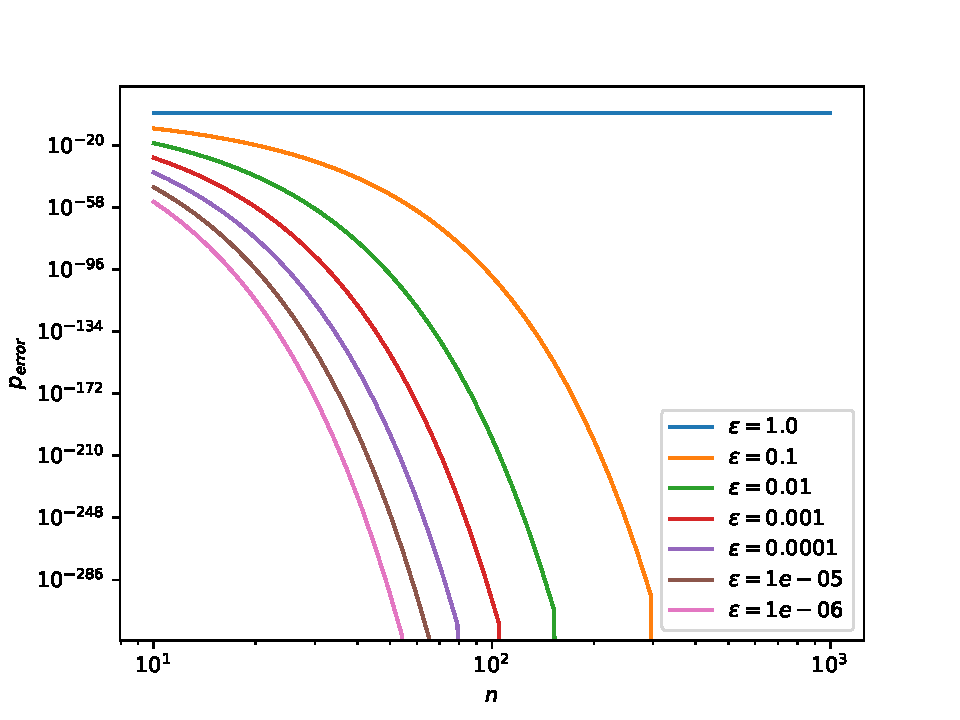
\includegraphics[width=0.8\textwidth]{figures/perrorplot.pdf}
%     \end{figure}

% \end{frame}

% \begin{frame}
%     \frametitle{Quantum SVM --- Bound plots}

%     \begin{figure}
%         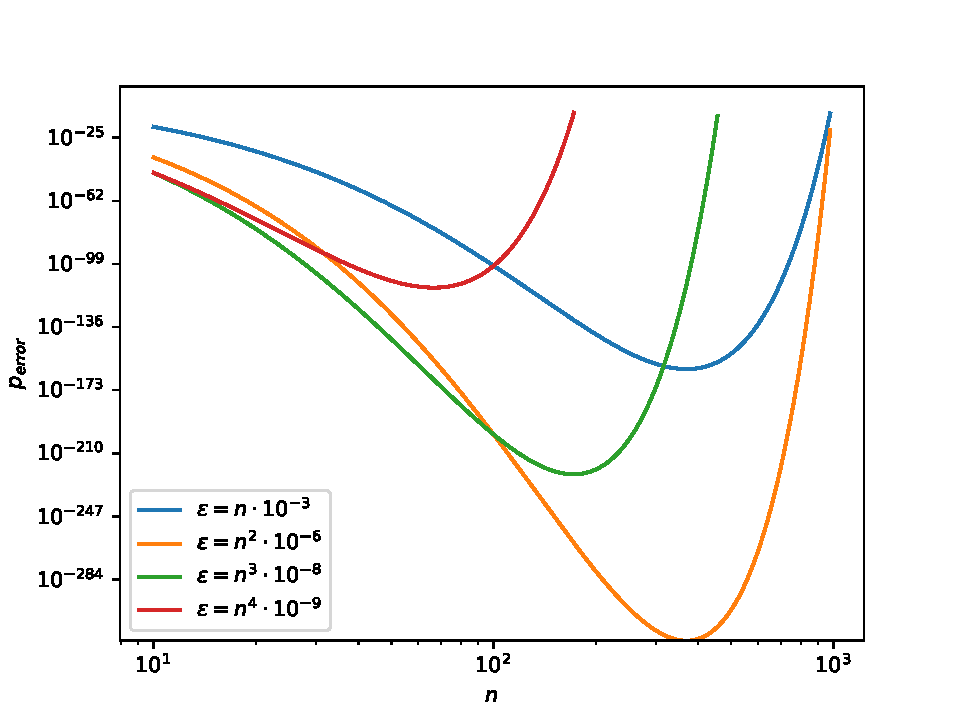
\includegraphics[width=0.8\textwidth]{figures/perrorscaled.pdf}
%     \end{figure}

% \end{frame}